% Created 2012-07-06 Fr 19:17
\documentclass[11pt]{article}
\usepackage[utf8]{inputenc}
\usepackage[T1]{fontenc}
\usepackage{fixltx2e}
\usepackage{graphicx}
\usepackage{longtable}
\usepackage{float}
\usepackage{wrapfig}
\usepackage{soul}
\usepackage{textcomp}
\usepackage{marvosym}
\usepackage{wasysym}
\usepackage{latexsym}
\usepackage{amssymb}
\usepackage{hyperref}
\tolerance=1000
\usepackage{color}
\usepackage{listings}
\providecommand{\alert}[1]{\textbf{#1}}

\title{Example}
\author{Bernd Weiss}
\date{2012-07-06}
\hypersetup{
  pdfkeywords={},
  pdfsubject={},
  pdfcreator={Emacs Org-mode version 7.8.11}}

\begin{document}

\maketitle

\setcounter{tocdepth}{3}
\tableofcontents
\vspace*{1cm}


\definecolor{dkgreen}{rgb}{0,0.5,0}
\definecolor{dkred}{rgb}{0.5,0,0}
\definecolor{gray}{rgb}{0.5,0.5,0.5}

\lstset{basicstyle=\ttfamily\bfseries\footnotesize,
morekeywords={virtualinvoke},
%%keywordstyle=\color{blue},
%%ndkeywordstyle=\color{red},
commentstyle=\color{dkred},
%%stringstyle=\color{dkgreen},
numbers=left,
numberstyle=\ttfamily\tiny\color{gray},
stepnumber=1,
numbersep=10pt,
backgroundcolor=\color{white},
tabsize=4,
showspaces=false,
showstringspaces=false,
xleftmargin=.23in
}


\begin{abstract}
abstract abstract abstract abstract abstract abstract abstract abstract abstract 
\end{abstract}


\section{Introduction and some R code}
\label{sec-1}


Let's start with an equation: 

\begin{equation}
v^{*}_{j} = v_{j} + \tau^{2} 
\end{equation}

Now, some R code:


\lstset{language=R}
\begin{lstlisting}
## Create 100 normally distributed numbers 
x <- rnorm(100)
## Estimate mean
mean(x)
sd(x)
var(x)
\end{lstlisting}

\begin{verbatim}
 [1] -0.01011993
 [1] 1.023805
 [1] 1.048176
\end{verbatim}

The mean of x is -0.01 -0.005
\section{Plot a histogram}
\label{sec-2}




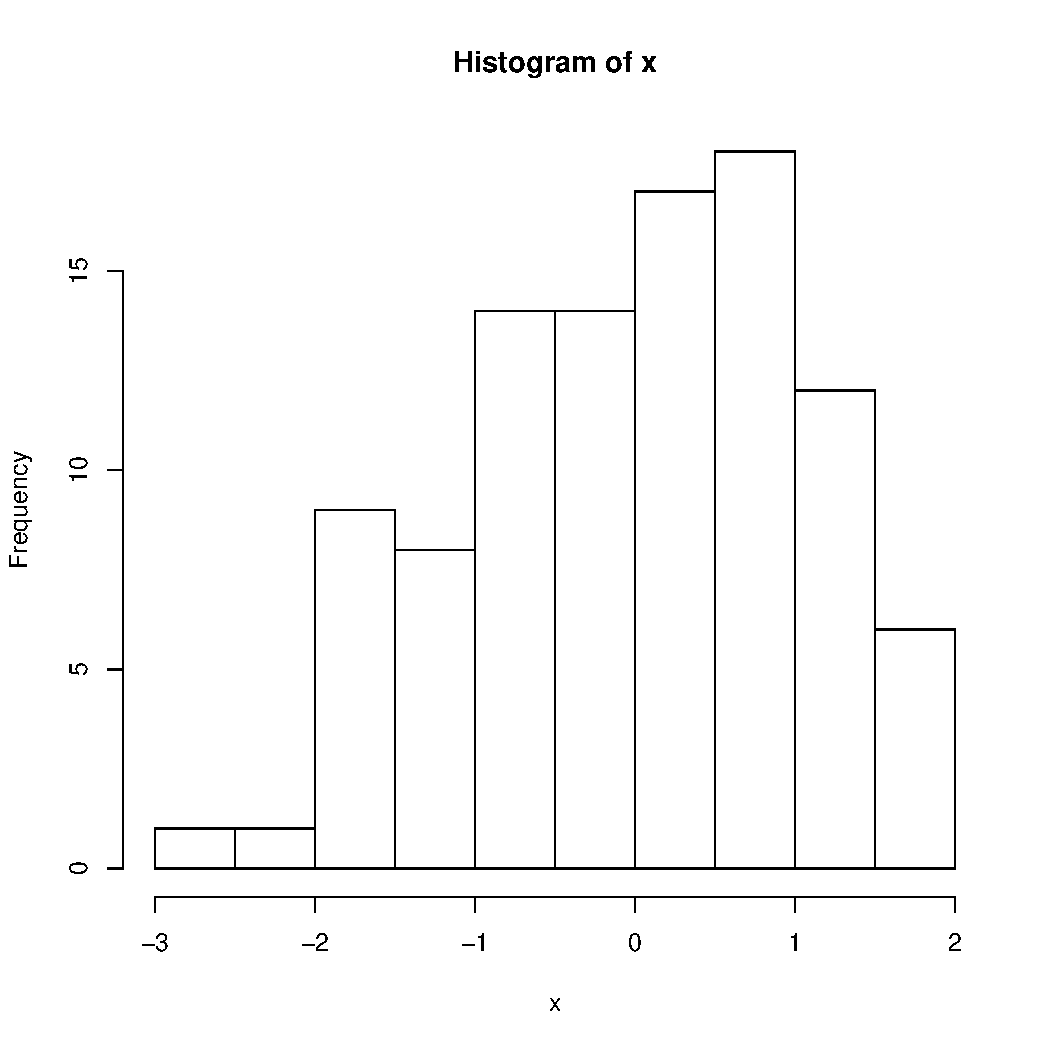
\includegraphics[width=.9\linewidth]{../fig/f_pub_histogram.pdf}





\begin{figure}[htb]
\centering
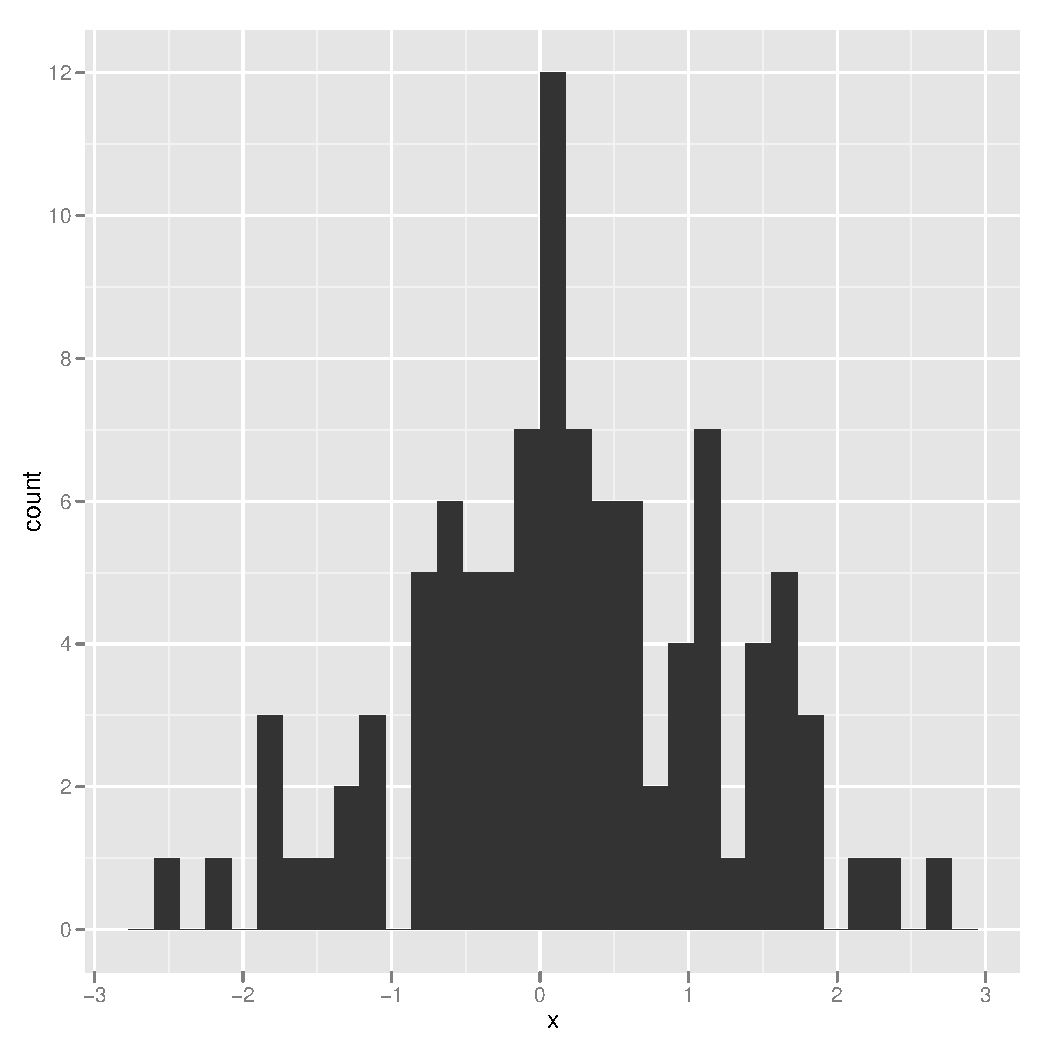
\includegraphics[width = 0.2\linewidth, clip]{../fig/f_pub_histogram_gg.pdf}
\caption{\label{f:ggplot}A beautiful ggplot2 plot}
\end{figure}

See Figure \ref{f:ggplot} blablabla
\section{Use the Bash!}
\label{sec-3}




\begin{verbatim}
 
 null device 
           1
 > total 248
 d--------- 1 weiss mkgroup      0 Jul  6 11:30 auto
 ---------- 1 weiss mkgroup    122 Jul  6 19:15 d_example.html
 ---------- 1 weiss mkgroup   2451 Jul  6 19:15 d_example.org
 ---------- 1 weiss mkgroup 238121 Jul  6 12:34 d_example.pdf
 ---------- 1 weiss mkgroup   2847 Jul  6 12:33 d_example.tex
\end{verbatim}



\lstset{language=R}
\begin{lstlisting}
substr(x, 1, 30)
\end{lstlisting}

\begin{verbatim}
 [1] "total 248\nd--------- 1 weiss m"
\end{verbatim}

\end{document}
